\documentclass[compileTAMUreport.tex]{subfiles}

\begin{document}

\section{Procedure followed in achieving the goal:}
\begin{itemize}
\item After doing an extensive literature review. We have narrowed the main parameter that have to be taken into account for getting the overall effectiveness of the model.
\item The first thing that we did was to model the individual cell of the metal foam. The shape of the cell was a tetrakiadecaheadron (14 phases - 8 equilateral triangle and 6 octagons)as it was supposed to the ideal model proposed by Lord Kelvin which solves free surface energy minimization during the solidification of a liquid in a highly disperse gas.
\item The next step was to find out the structure of the individual filaments and node shape.

\begin{itemize}

\item We designed that the filament shape to be equilateral triangular prism, as it would simplify the calculation, we optimized the design in Solidworks using design studies so has to have the maximum porosity.
\item We designed the node to be spherical as it has the lowest volume to surface area ratio which would enhance the heat transfer between the node and the fluid.
\end{itemize}


\item After modeling the cell structure we had to find out all the various Inlet properties and dimesionalless numbers like reynold and prandtln number For which we used the EES software.
\item	The next step was to find the plane of symmetry in the cell structure we constructed so as to the simply the problem to some level. Solving this we ended up the model shown in the figure below. (figure)
\item The surface area of the foam in contact with the tube was calculated using the pore density, the geometric density of spheres to prism faces such that on average 3.2 faces per cell will intersect the wall. The most area on average that will intersect the wall is $(\pi D^2)/4$ for the spheres and $0.5 a^2 \cos (30)/ \cos(54.7)$ for the equilateral triangle, and the least area would always be the cross section of the equilateral triangle: $a^2 * \cos(30) $ Given the assumed structured nature of the foam, it is acceptable to average the maximum and minimum areas for the for number of foam cells that lie on the tube interface. The number of pores that could be intersected is $PPI\cdot\pi D$. 
\item	Now we calculated the heat transfer between the two nodes and the filament assembly while the fluid is being passed.
\item After constructing the temperature profile between nodes along the filament, we constructed the temperature profile in the radial direction. We constructed the model by taking the boundary conditions to be 
\begin{itemize}

\item Temperature at the surface of the boiler to be a constant value as stated in the assumptions.
\item Temperature at the center of the boiler piper to the local saturation temperature which varies on the local pressure (pressure profile).
\end{itemize}

\begin{figure}[t]
\begin{center}
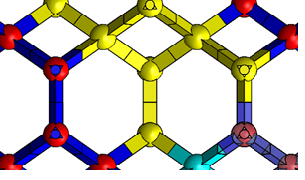
\includegraphics[width=0.75\textwidth]{./figure/Resistance1}
\end{center}
\caption{Resistance Circuit At 0°}
\label{fig:flowregime}
\end{figure}
\item	Constructed the profile for the quality of steam along the length of the boiler using 
\item	Then we constructed the pressure profile along the length of the tube as there will be a pressure drop due to the presence of the metal foam.  We used the Forschimer Darcy model \cite{Xu2012}

\item Using the above temperature profile we constructed the relation between the length of the pipe and the quality factor. As we have stated in the assumption that we have limited the quality of steam to be 0.8.
\end{itemize}
\end{document} 
